\subsection{Trafo Vol 1.0}
Gegeben sind folgende Daten:
\begin{itemize}
\itemsep0em
\item Primärspannung $U_1 = 32kV$, Sekundärspannung $U_2 = 400V$
\item Scheinleistung des Trafos $S = 1MVA$
\item Fläche des Eisenkerns $A_{FE} = 0.05m^2$
\item Maximale Flussdichte des Eisens $\hat{B} = 1.8T$
\item Streureaktanzen $X_{\sigma 1} = 30\Omega$, $X_{\sigma 2} = 7m\Omega$ 
\end{itemize}
\begin{enumerate}
\item Berechnen sie die Anzahl Windungen der Primär und Sekundärwicklung
\begin{align*}
U_{10} = \frac{2\pi}{\sqrt{2}} N_1\cdot f\cdot \hat{B} \cdot A_{FE} \Rightarrow N_1&= \frac{U_{10}\cdot \sqrt{2}}{2\cdot \pi \cdot f\cdot \hat{B} \cdot A_{FE}} &&= \frac{32'000V\cdot \sqrt{2}}{2\pi\cdot 50\cdot 1.8T\cdot 0.05m^2}=1600.56 \textrm{ Windungen}\approx	1601\\
N_2 &= \frac{U_{20}\cdot \sqrt{2}}{2\cdot \pi\cdot f\cdot \hat{B}\cdot A_{FE}}&&=\frac{400V\cdot \sqrt{2}}{2\pi\cdot 50\cdot 1.8T\cdot 0.05m^2}=20 \textrm{ Windungen}
\end{align*}
	
\item Berechnen sie den Primär und Sekundärstrom
\begin{align*}
I_1&=\frac{P}{U_1} &&=\frac{1\cdot10^6VA}{32'000V} = 31.25A\\
I_2&=\frac{P}{U_2} &&=\frac{1\cdot10^6VA}{400V} = 2500A
\end{align*}

\item Berechnen sie die Wicklungsverluste über der Primär und Sekundärwicklung wenn der Primärwiderstand $R_{10} = 20\Omega$ und der Sekundärwiderstand $R_{20} = 8m\Omega$ beträgt
\[
	P_W = P_{W1} + P_{W2} = I_1^2\cdot R_1+I_2^2\cdot R_2 = (31.25A)^2\cdot 20\Omega +(2500A)^2\cdot 0.008\Omega = 19.531kW+50kW = 69.531kW
\]
Wichtig: Über den Strom rechen da die Spannung auch den magnetischen Teil enthält der nicht in Wärme umgesetzt wird.

\item Berechnen sie den Wirkungsgrad des Transformators im Nennbetrieb wenn die Leerlaufleistung $P_L = 30kW+j\cdot 40kVAr$
\[
	\eta = \frac{P_{ab}}{P_{zu}} = \frac{S-P_W-P_L}{S} = \frac{1000kW-69.531kW-30.000kW}{1000kW} \cdot 100\%= 90.04\% 
\]

\newpage
\item Zeichen sie das Vollständige Zeigerdiagramm des Trafos bei Nennlast.

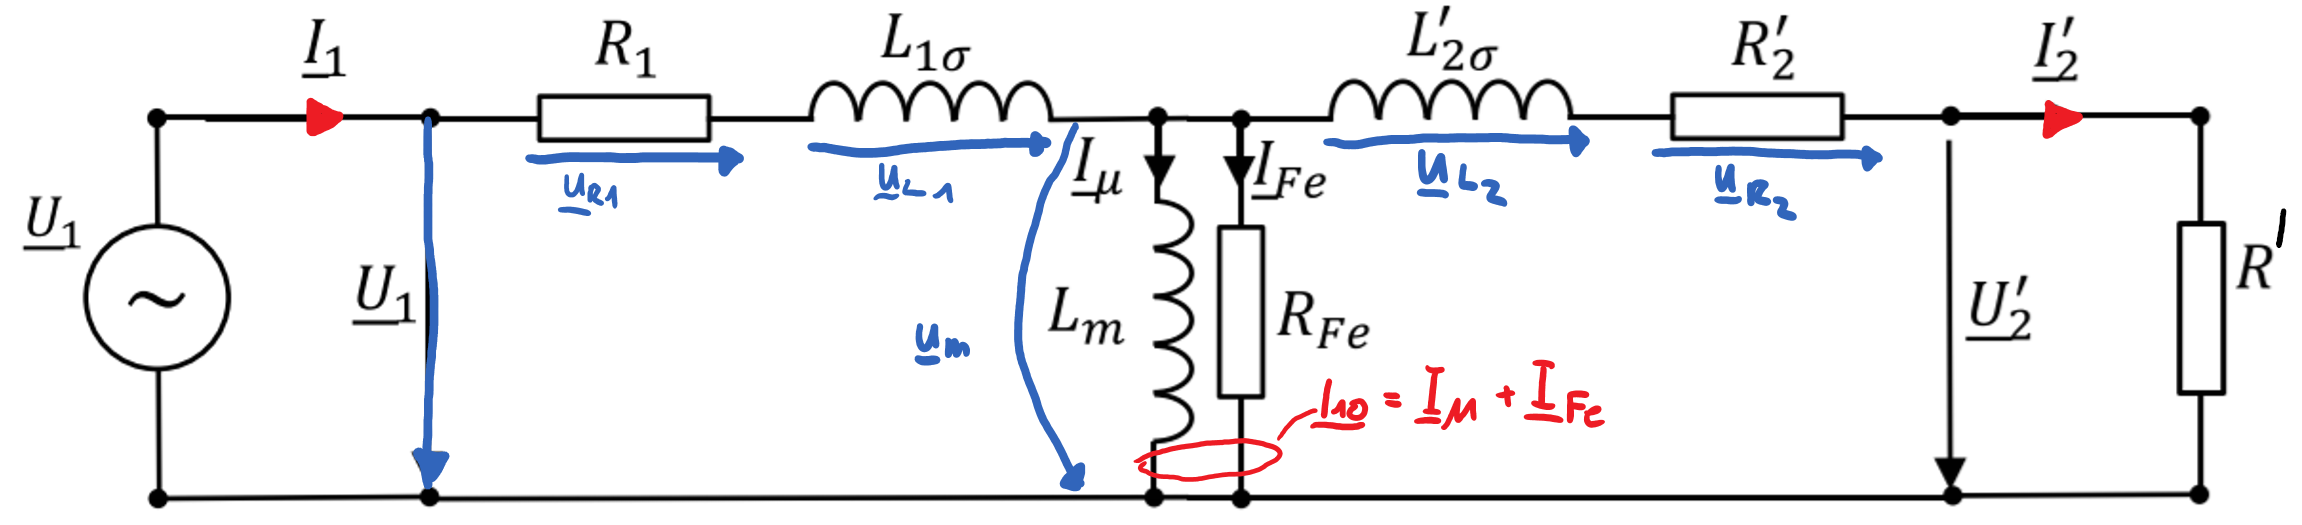
\includegraphics[width=0.99\textwidth]{bilder/a52.png}

\begin{minipage}{0.49\textwidth}
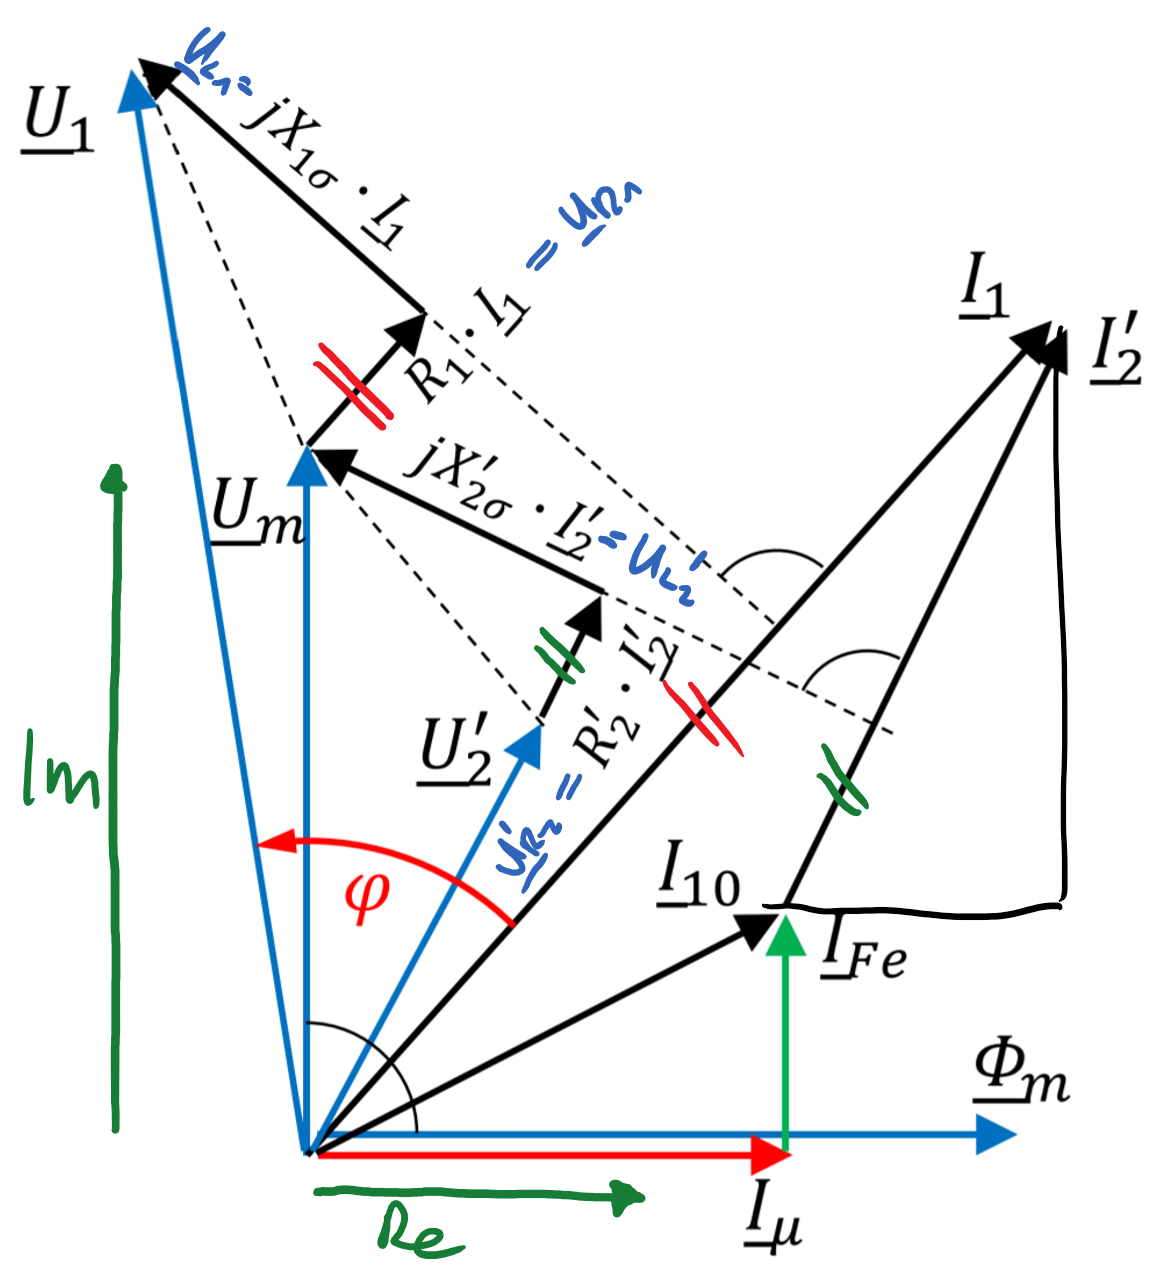
\includegraphics[width=0.7\textwidth]{bilder/a53.png}
\end{minipage}
\begin{minipage}{0.49\textwidth}
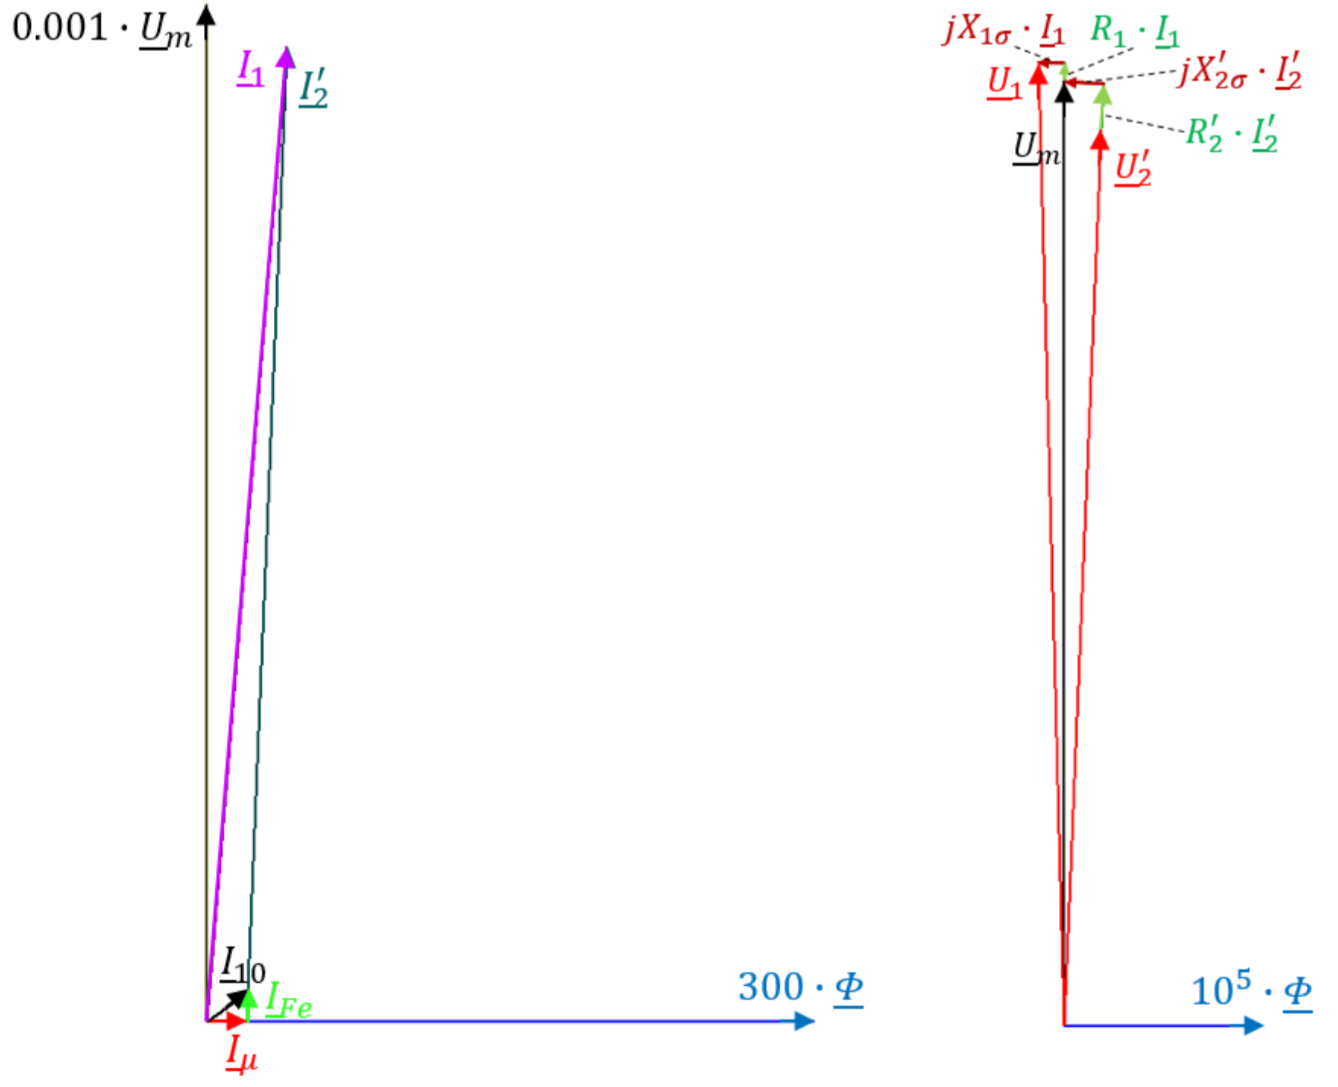
\includegraphics[width=0.9\textwidth]{bilder/a5.png}
\end{minipage}

\end{enumerate}


\begin{minipage}{0.4\textwidth}
Eigentlich ist der Fluss $\Phi_m$ reell und $U_m$ desshalb  $90^\circ$ verschoben (rein imaginär). Desshalb ist der Strom durch $R_{Fe}$ imaginär und durch $L_m$ reell!
\begin{enumerate}
	\itemsep0em 
	\item Alle Ströme und Spannungen gemäss Diagramm oben benamseln
	\item Maschengleichung 1: $\underline{U}_1 = \underline{U}_m+\underline{U}_{L1}+\underline{U}_{R1}$
	\item Maschengleichung 2: $\underline{U}_m=\underline{U}_{L2}'+\underline{U}_{R2}'+\underline{U}_2'$
	\item Knotengleichung 1:$\underline{I}_{10} = \underline{I}_\mu + \underline{I}_{Fe}$
	\item Knotengleichung 2:$\underline{I}_1 = \underline{I}_{10}
+ \underline{I}_{2}'$
	\item Zeigerdiagramm ausgehend von $\underline{U}_m$ auf der reellen Achse
	
\end{enumerate}
\end{minipage}
\begin{minipage}{0.59\textwidth}
\begin{align*}
	\underline{U}_1 &= j\cdot U_{10} = j\cdot 32kV\\
	\Phi_m&= \left(\frac{B\cdot A}{\sqrt{2}}\angle 0^\circ\right) = \left(\frac{1.8T\cdot 0.05m^2}{\sqrt{2}}\right) = 0.636Vs\\
	\hat{\underline{U}}_1 &= j\cdot \omega \cdot N_1\cdot B\cdot A_{Fe}\\
	I_{FE} &= j\cdot\frac{P_{FE}}{U_m} =j\cdot\frac{30kW}{32kV}=j\cdot 0,9375A\\
	I_\mu &= \frac{Q_u}{U_m} = \frac{40kVAr}{32kV} = 1.25A\\
	I_{10}&=I_{FE}+I_{\mu} = j\cdot 0.9375A+1,25A = (1.562A\angle 36.87^\circ)\\
	R_L &= \frac{P_N}{I_2^2} = \frac{10^6 VA}{(2500 A)^2}= 0.16\Omega \quad \textrm{Aus Nennlastbedingung}\\
	R_2' &= R_2\cdot  \left(\frac{N_1}{N_2}\right)^2=0.008\Omega\cdot\left(\frac{1600}{20}\right)^2= 51.2\Omega\\
	X_{\sigma 2}' &=X_{\sigma 2}\cdot \left(\frac{N_1}{N_2}\right)^2=0.007\Omega\cdot\left(\frac{1600}{20}\right)^2=  44.8\Omega\\
	I_2'&= \frac{\underline{U}_1}{\left(\frac{N_1}{N_2}\right)^2\cdot \left(R_L+ R_2+jX_{\sigma 2}\right) }\\
	& = \frac{j\cdot 32kV }{\left(\frac{1600}{20}\right)^2\cdot \left(0.16+0.008+j 0.007\right)\Omega} = 1.238+j\cdot 29.710\\
	I_1&=I_2'+I_\mu+I_{FE} = 1.238+j\cdot 29.710+1.25A+j\cdot 0.9375A\\
	&= (2.488+j\cdot 30.647)A
\end{align*}
\end{minipage}
\[
	\begin{array}{llll}
		U_1 &= R_1\cdot \underline{I}_1 + jX_{\sigma 1}\cdot  \underline{I}_1+\underline{U}_m &= (20 +j\cdot 30)\Omega\cdot (2.488+j\cdot 30.647)A+j\cdot 32'000V &= (-869+j\cdot 32786.6)V\\
		U_2 &= \underline{U}_m - R_2'\cdot \underline{I}_2' + jX_{\sigma 2}' \underline{I}_2' &= j\cdot 32'000V-(51.2 + j\cdot 44.8)\Omega \cdot (1.238+j\cdot 29,710)A&= (1267,622+j\cdot 30'423.386)V
	\end{array}	
\]
